% !TeX root = ../../script.tex
\documentclass[../../script.tex]{subfiles}

\begin{document}
\section{Function Sequences and Differentiability}

\begin{eg}
    Consider $\seq{f}$:
    \begin{align*}
        f_n: \realn &\longrightarrow \cmpln \\
        x &\longmapsto \frac{1}{n} e^{inx}
    \end{align*}
    Then 
    \begin{gather*}
        \supnorm{f_n} = \frac{1}{n} \conv{} 0 \\
        \iff\\
        \seq{f} \text{ converges uniformly to the zero function}
    \end{gather*}
    But 
    \[
        f_n'(x) = ie^{inx} = i(e^{ix})^n
    \]
    converges (pointwise even) only for $x = 2k\pi, ~~k \in \intn$.
\end{eg}

\begin{rem}
    Let $f: X \rightarrow V$ where $V$ is a normed vector space. Define 
    \[
        \supnorm{f} = \sup\set[x \in X]{\norm{f(x)}}
    \]
    the supermum norm. Also define 
    \begin{itemize}
        \item $B(X, V)$ the space of bounded functions from $X \rightarrow V$
        \item $C_B(X, V)$ the space of continuous, bounded functions from $X \rightarrow V$
    \end{itemize}
\end{rem}

\begin{thm}
    Let $U \subset \realn^n$ be open and $f_n: U \rightarrow \realn^m$ continuously differentiable $\forall n \in \natn$.
    If $\seq{f}$ and $(Df_n)$ converge uniformly to $f: U \rightarrow \realn^m$ and $g:U \rightarrow \realn^{m \times m}$,
    then $f$ is differentiable and $Df = g$.
\end{thm}
\begin{proof}
    First consider $m = 1$. We use the operator norm on $\realn^{m \times m}$.
    First, let $Df_n$ be continuous $\forall n$ and thus $g$ is continuous.
    Choose $x \in U$ and $\epsilon > 0$, then 
    \begin{equation}
        \exists \delta > 0: ~~\norm{g(y) - g(x)} < \frac{\epsilon}{3} ~~\text{ if }~~ \norm{y - x} < \delta
    \end{equation}
    Furthermore 
    \begin{equation}
        \exists N \in \natn: ~~\supnorm{Df_n - g} < \frac{\epsilon}{3} ~~\forall n > N
    \end{equation}
    Let $y \in \oball[\delta](x)$. Then according to the intermediate value theorem,
    \begin{equation}
        \forall n \in \natn ~\exists \xi_n \in \oline = \set[{t \in [0, 1]}]{x + t(y - x)}
    \end{equation}
    such that 
    \begin{equation}
        f_n(y) - f_n(x) = Df_n(\xi_n)(y - x)
    \end{equation}
    We have $\xi_m \in \oball[\delta](x)$. Then 
    \begin{equation}
        \begin{split}
              &\frac{1}{\norm{y - x}} \left| f_n(y) - f_n(x) - Df_n(x)(y - x) \right| \\ 
            = &\frac{1}{\norm{y - x}} \underbrace{\abs{(Df_n(\xi_n) - Df_n(x))(y - x)}}_{\norm{Df_n(\xi_n)} - Df_n(x)\norm{y - x}} \\
            \le &\norm{Df_n(\xi_n) - Df_n(x)} \\
            \le &\norm{Df_n(\xi_n) - g(\xi_n)} + \norm{g(\xi_n) - g(x)} + \norm{g(x) - Df_n(x)} \\
            \le &\supnorm{Df_n - g} + \norm{g(\xi_n) - g(x)} + \supnorm{g - Df_n} \\
            = &2\supnorm{Df_n - g} + \norm{g(\xi_n) - g(x)} < \epsilon
        \end{split}
    \end{equation}
    For $n \rightarrow \infty$ we have 
    \begin{equation}
        \frac{1}{\norm{y - x}} \abs{f(y) - f(x) - g(x)(y - x)} < \epsilon ~~\forall y \in \oball[\delta](x)
    \end{equation}
    Since $\epsilon > 0$ is arbitrary, we get 
    \begin{equation}
        \limes{y}{x} \frac{1}{\norm{y - x}} \abs{f(y) - f(x) - g(x)(y - x)} = 0
    \end{equation}
    This means that $f$ is differentiable in $x$ with $Df(x) = g(x)$.
\end{proof}

\begin{rem}
    On $C_B^1(U, \realn^m)$ (the space of continuous, differentiable and bounded functions with bounded derivative) we can define a norm:
    \[
        \cnorm{f} := \supnorm{f} + \supnorm{Df}
    \]
    Then the above theorem is equivalent to the statement that $C_B^1(U, \realn^m)$ with $\cnorm{f}$ is complete.
\end{rem}

\begin{thm}
    Let $f(x) = \sum_{n=0}^{\infty} a_n x^n$ be a power series with positive convergence radius $\rho$.
    Then $f$ is differentiable on $\oball[\rho](0)$ and 
    \[
        f'(x) = \sum_{n=0}^{\infty} n a_n x^{n-1}
    \]
\end{thm}
\begin{proof}
    We need to inspect the convergence radius $R$ of 
    \begin{equation}
        \sum_{n=0}^{\infty} n a_n x^{n-1} = \frac{1}{x} \sum_{n=0}^{\infty} n a_n x^{n}
    \end{equation}
    $(\sqrt[n]{n})$ converges to $1$, so $\exists \epsilon > 0$ such that for sufficiently big $n$ we have 
    \begin{equation}
        (1 - \epsilon)\sqrt[n]{a_n} \le \sqrt{n a_n} \le (1 + \epsilon)^n \sqrt{a_n}
    \end{equation}
    and thus 
    \begin{equation}
        \frac{1 - \epsilon}{\rho} = (1 - \epsilon) \cdot \limsupn \sqrt[n]{\abs{a_n}} \le \limsupn \sqrt[n]{\abs{n a_n}} = \frac{1}{R} \le \frac{1 + \epsilon}{\rho}
    \end{equation}
    So 
    \begin{equation}
        \implies \frac{1 - \epsilon}{\rho} \le \frac{1}{R} \le \frac{1 + \epsilon}{\rho}
    \end{equation}
    Since this holds for every $\epsilon$, this implies $\rho = R$. 
    Now for $x \in \oball[\rho](0)$ set
    \begin{equation}
        g(x) := \series{k} n a_n x^{n - 1}
    \end{equation}
    Let $x \in \oball[\rho](0)$ be fixed and choose $a > 0$ such that $\abs{x} < a < \rho$.
    This means that 
    \begin{align*}
        f_N(x) := \sum_{n=0}^{N} a_n x^n && \text{and} && g_N(x) := \sum_{n=0}^{N} a_nx^{n-1}
    \end{align*}
    converge uniformly on $\oball[a](0)$ to $f$ and $g$.
    Obviously, $f_N' = g_N$, so $f$ is differentiable and $f' = g$.
    Since differentiabiility is a local property, the desired statement follows $\forall x \in \oball[\rho](0)$.
\end{proof}

\begin{cor}
    Let $f(x) = \sum_{n=0}^{\infty} a_n x^n$ be a power series with convergence radius $\rho > 0$. Then $f \in C^{\infty}(\oball[r](0))$, and 
    \[
        a_k = f^{(k)}(0) \cdot \inv(k!)
    \]
    Furthermore, the series representation (if it exists) is unique.
\end{cor}
\begin{proof}
    The infinite Differentiability follows inductively from the previous theorem. Also inductively we have 
    \begin{equation}
        f^{(k)}(x) = \sum_{n=0}^{\infty} n(n-1) \cdots (n - k + 1) a_nx^{n-k}
    \end{equation}
    Choose $x = 0$ and receive 
    \begin{equation}
        f^{(k)}(0) = n (n-1) \cdots (n - k + 1) a_n
    \end{equation}
\end{proof}

\begin{eg}[Derivative of the exponential function]
    \[
        (e^x)' = \sum_{n=0}^{\infty} \left(\frac{x^n}{n!}\right)' = \sum_{n=1}^{\infty} \frac{n x^{n-1}}{n!} = \sum_{n=1}^{\infty} \frac{x^{n-1}}{(n-1)!} = \sum_{n=0}^{\infty} \frac{x^n}{n!} = e^x
    \]
\end{eg}

\begin{rem}[Taylor Series]
    We can define the Taylor series for $f: \field \rightarrow \field$
    \[
        \sum_{n=0}^{\infty} \frac{f^(n)(0)}{n!} x^n = f(x)
    \]
    \begin{itemize}
        \item In general, this doesn't hold true for all $x$, not even for $f \in C^{\infty}$.
        \item The convergence radius could be $0$
        \item There are examples of convergent Taylor series that don't converge to the initial function, e.g.
        \[
            f: x \mapsto \begin{cases}
                \exp\left(-\frac{1}{x}\right), & x > 0 \\
                0, & \text{else}
            \end{cases}
        \]
        $f$ is infinitely continuously differentiable in $0$, but the Taylor series would converge to $0$.
    \end{itemize}
\end{rem}

\begin{defi}
    Let $a_{\eta} \in \field$ (Multiindex notation) be coefficients $\forall \eta \in \natn_0^d$. Then 
    \[
        \sum_{\eta \in \natn_0^d} a_{\eta} x^{\eta}
    \]
    is said to be a (formal) power series with $d$ variables.
    
    A function $f: U \rightarrow \field$ with $U$ neighbourhood around $0$ is said to be analytic in $0$, if and only if 
    \[
        \exists \epsilon > 0, a_{\eta} \in \field: ~~f(x) = \sum_{\eta \in \natn_0^d} a_{\eta} x^{\eta} ~~\forall x \in \oball(0)
    \]
\end{defi}

\begin{rem}
    \begin{enumerate}[(i)]
        \item The convergence of the series to $S(x)$ can be defined as follows: 
        $\forall \epsilon > 0 ~\exists A \subset \natn_0^d \text{ finite}$ such that $\forall B \supset A$ finite we have 
        \[
            \abs{\sum_{\eta \in B} a_{\eta} x^{\eta} - S(x)} < \epsilon
        \]

        \item If the series converges in $(y_1, \cdots, y_n)$, then it also absolutely converges in the open cuboid 
        \[
            \set[\abs{x_i} < \abs{y_i} ~~\forall i \in \set{1, \cdots, d}]{x \in \realn^d}
        \]
        which means 
        \[
            \sum_{\eta \in \natn_0^d} \abs{a_{\eta}} (\abs{x_1}, \cdots, \abs{x_d})^{\eta} < \infty
        \]

        \item If the power series converges on a neighbourhood $U$ around $0$, then it is infinitely differentiable and 
        \[
            a_{\eta} = \frac{\partial^{\eta} f(0)}{\eta!}
        \]
        with 
        \begin{align*}
            \partial^{\eta} := \partial_1^{\eta_1} \partial_2^{\eta_2} \cdots \partial_d^{\eta_d} && \eta! := \eta_1! \eta_2! \cdots \eta_d!
        \end{align*}

        \item The formula above is only rarely useful to calculate the Taylor series. By inverting it we can calculate the 
        derivative of a known series representation. E.g.
        \[
            f(x) = xe^{x^2} = x \cdot \sum_{k = 0}^{\infty} \frac{(x^2)^k}{k!} = \series_{k=0}^{\infty} \frac{x^{2k + 1}}{k!} ~~\forall x \in \field
        \]
        $f^{(k)}(0) = 0$ is $k$ is even, and it is something else if $k$ is odd.

        \item $C^{\omega}(U)$ is the space of all analytic functions.
        \[
            C(U) \supset C^1(U) \supset C^2(U) \supset \cdots \supset C^k(U) \supset \cdots \supset C^{\infty}(U) \supset C^{\omega}(U)
        \]

        \item The analytic functions are closed among sums, products and concatinations. 
        A power series is analytic within its converges radius.
    \end{enumerate}
\end{rem}

\begin{eg}
    Consider the power series 
    \[
        \sum_{n=0}^{\infty} (xy)^n = \sum_{\eta \in \natn_0^2} (x y)^{\eta} \cdot a_{\eta}
    \]
    with 
    \begin{align*}
        &a_{\eta} = 1 \text{ if } \eta_1 = \eta_2 \\
        &a_{\eta} = 0 \text{ else}
    \end{align*}
    This series converges on 
    \[
        \set[\abs{xy} < 1]{(x, y)}
    \]
    to $\frac{1}{1 - xy}$.

    \begin{center}
        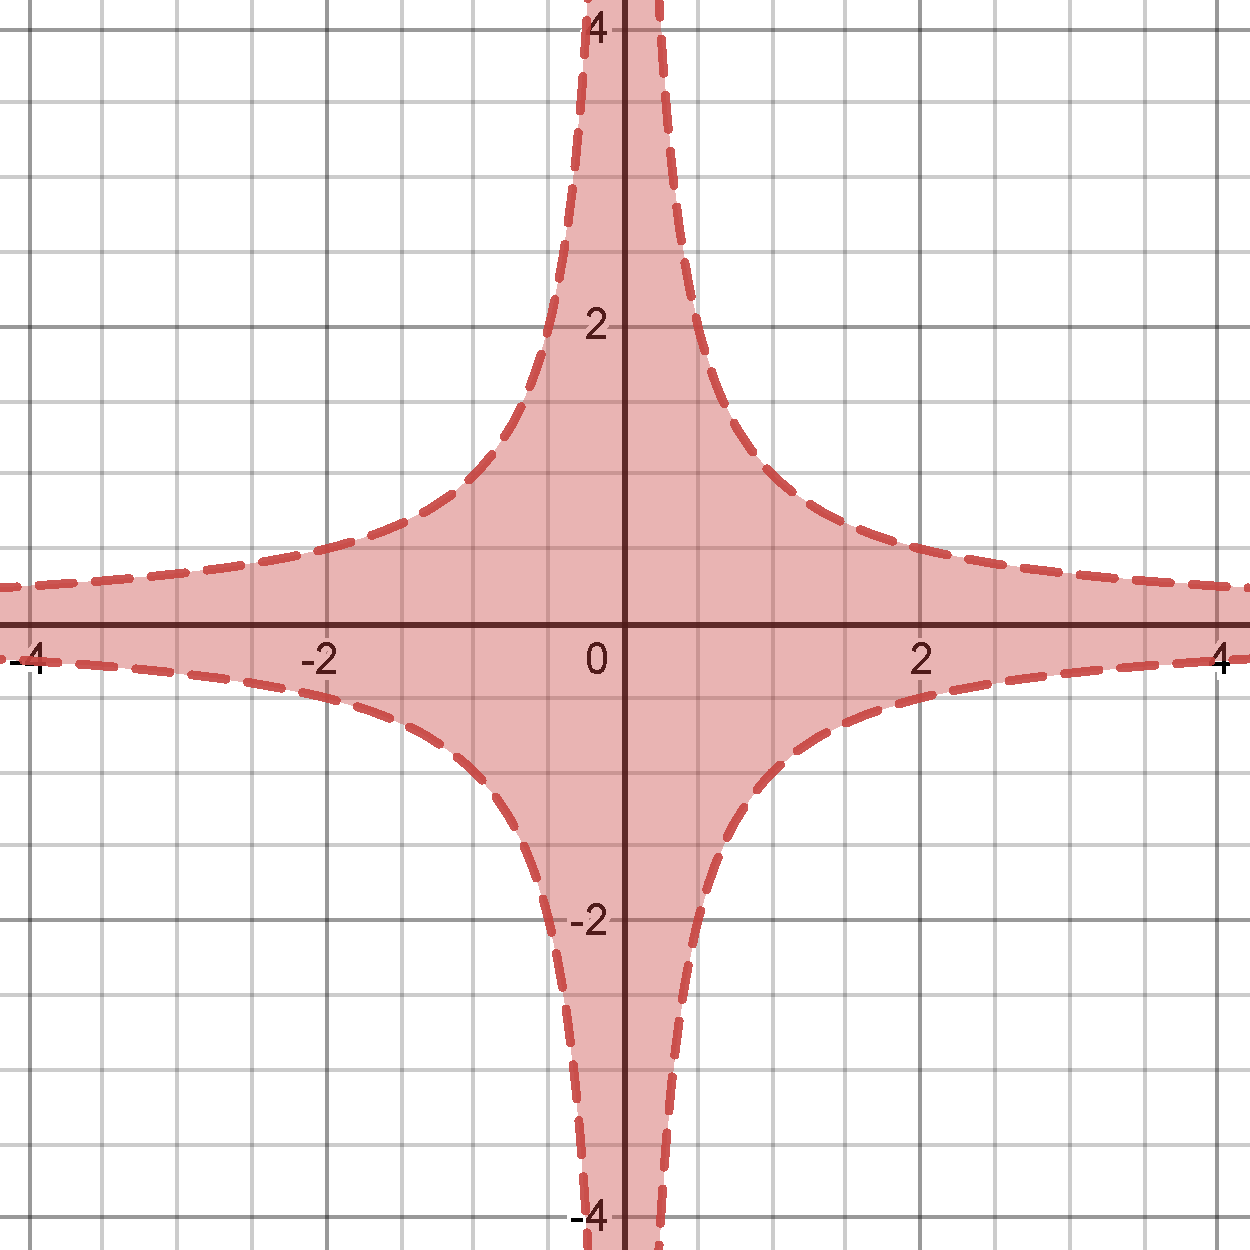
\includegraphics[scale=0.5]{../../assets/conv_rad.pdf}
    \end{center}

    So the convergence area must not necessarily be a sphere. The limit function is also defined outside of the convergence area.
\end{eg}
\end{document}